%%%%%%%%%%%%%%%%%%%%%%%%%%%%%%%%%%%%%%%%%%%%%%%%%%%%%%%%%%%%%%%
\documentclass{beamer}
\usecolortheme{whale}
\setbeamersize{text margin left=5mm,text margin right=5mm}

% Used to create a section slide between section
\AtBeginSection[]{
  \begin{frame}
  \vfill
  \centering
  \begin{beamercolorbox}[sep=8pt,center,shadow=true,rounded=true]{title}
    \usebeamerfont{title}\insertsectionhead\par%
  \end{beamercolorbox}
  \vfill
  \end{frame}
}
%%%%%%%%%%%%%%%%%%%%%%%%%%%%%%%%%%%%%%%%%%%%%%%%%%%%%%%%%%%%%%%

% Title page

\title{Stroke Audit Machine Learning (SAMueL) \\ Workshop 1}
\subtitle{Investigating variation in clinical decision-making with explainable AI}


\author{Kerry Pearn\inst{1}, Keira Pratt-Boyden\inst{1}, Martin James\inst{1,2}, Michael Allen\inst{1}}
\institute{\inst{1} University of Exeter Medical School \inst{2} Royal Devon University Healthcare NHS Foundation Trust}

%\institute{Overleaf}
\date{November 2022}


\begin{document}

\frame{\titlepage}

%%%%%%%%%%%%%%%%%%%%%%%%%%%%%%%%%%%%%%%%%%%%%%%%%%%%%%%%%%%%%%%

\begin{frame}
\frametitle{Breaking down the emergency stroke pathway into key steps}
\begin{center}
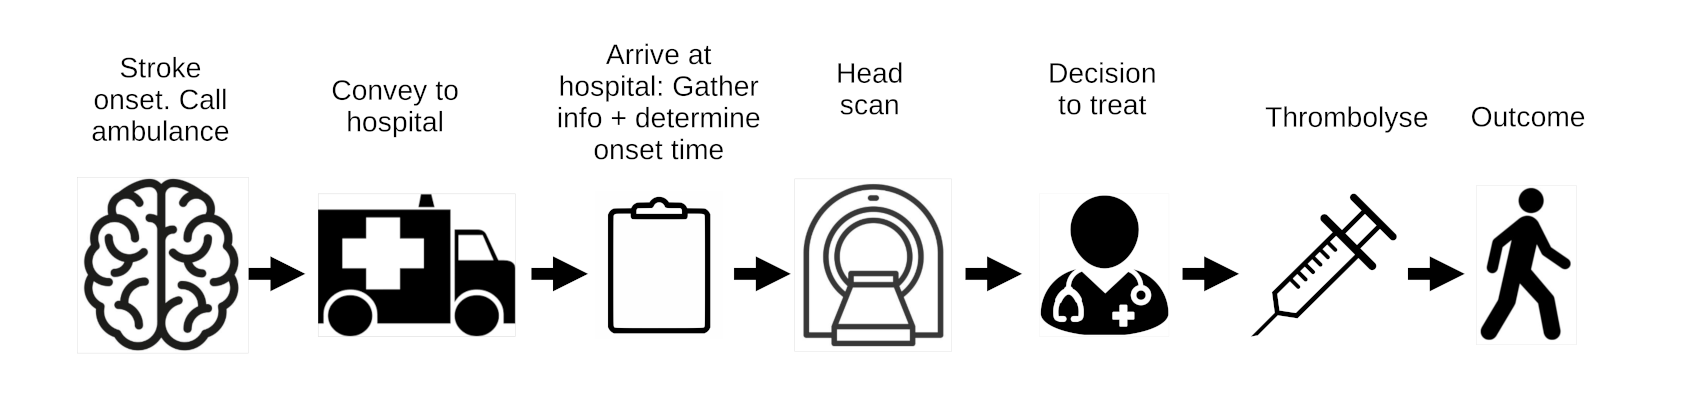
\includegraphics[width=1.0\textwidth]{./images/pathway}
\end{center}
We can model key changes to pathway:
\begin{itemize}
    \item What if the pathway were faster?
    \item What if hospital determined the stroke onset time in more patients?
    \item What if clinical decision-making was like that of \emph{benchmark} hospitals? (Predict what treatment a patient would receive at other hospitals).
\end{itemize}
\end{frame}

%%%%%%%%%%%%%%%%%%%%%%%%%%%%%%%%%%%%%%%%%%%%%%%%%%%%%%%%%%%%%%%

\begin{frame}
\frametitle{Machine learning overview}
\begin{center}
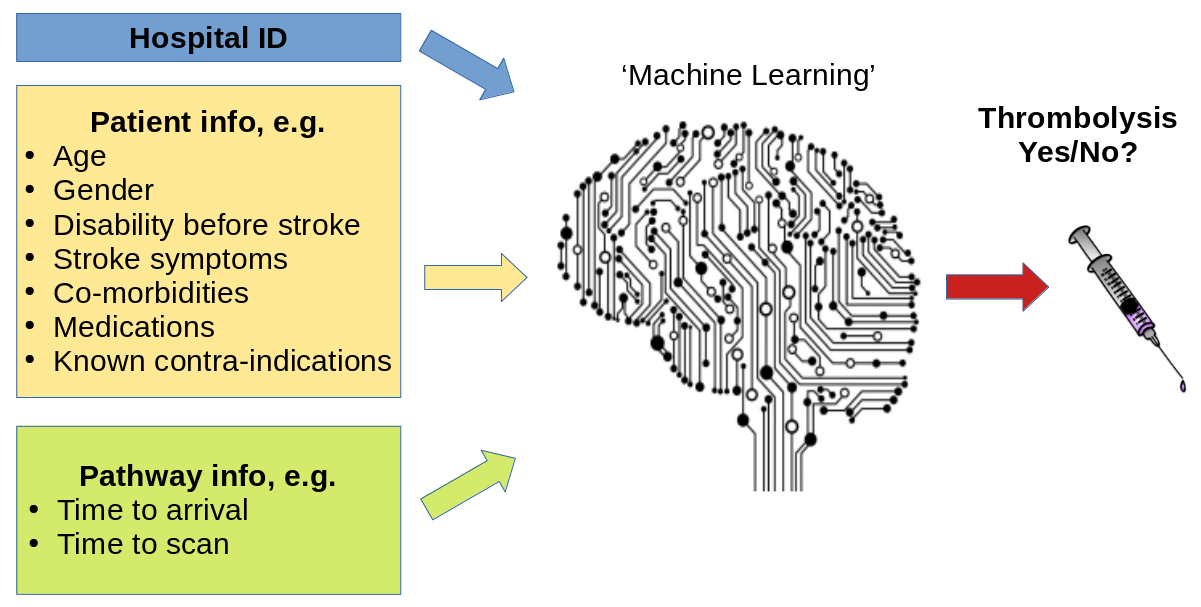
\includegraphics[width=0.95\textwidth]{./images/ml_model_high_level}
\end{center}

We accessed 240,000 emergency stroke admissions in England and Wales over three years.
\end{frame}


%%%%%%%%%%%%%%%%%%%%%%%%%%%%%%%%%%%%%%%%%%%%%%%%%%%%%%%%%%%%%%%

\begin{frame}
\frametitle{Explaining model predictions with SHAP values}

SHAP values show the influence of features (even for \emph{`black box'} models).

\begin{center}
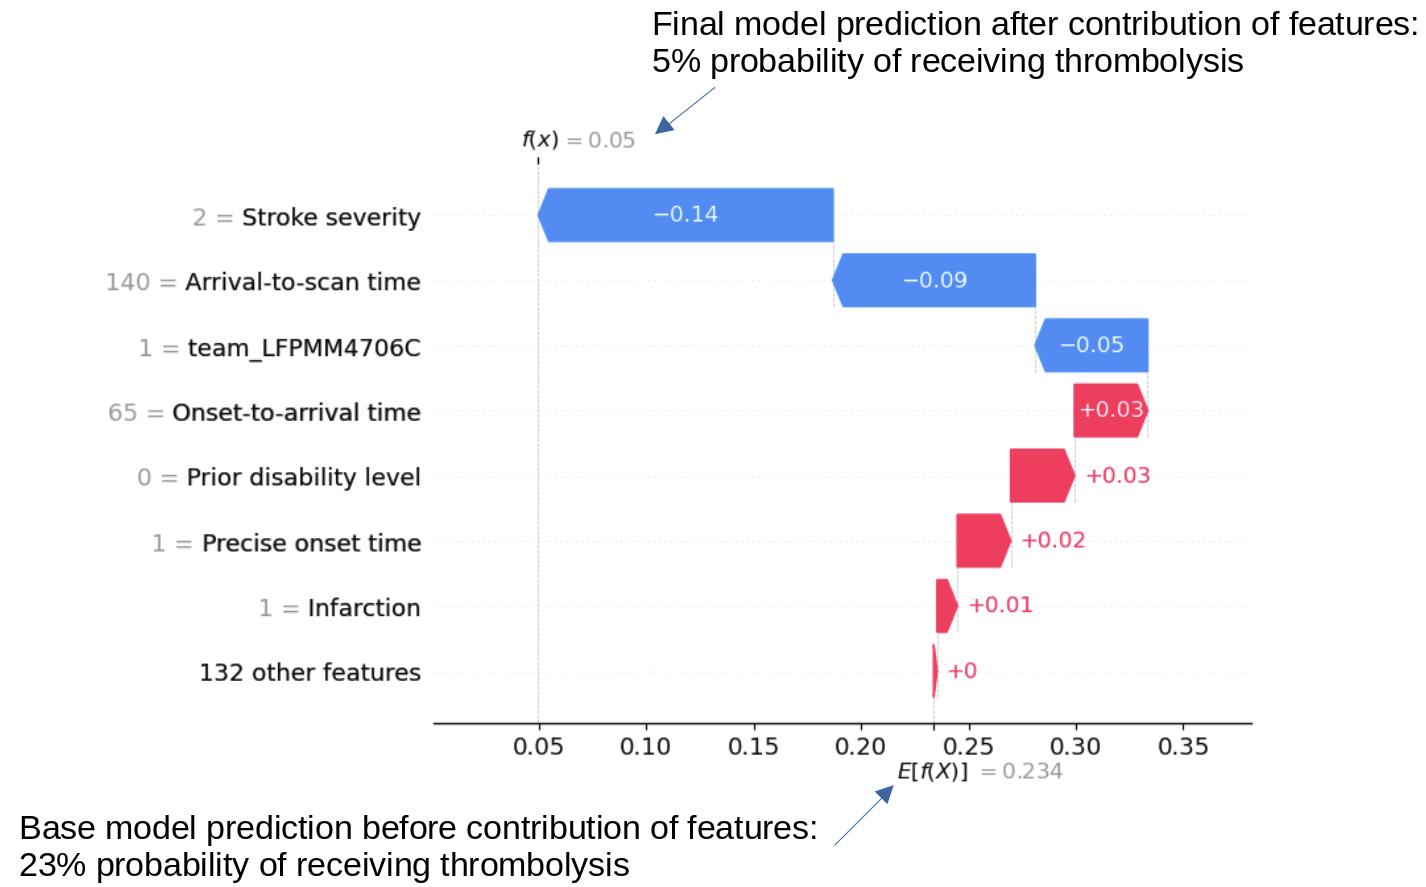
\includegraphics[width=0.83\textwidth]{./images/xgb_waterfall_low_probability.jpg}
\end{center}
\end{frame}


%%%%%%%%%%%%%%%%%%%%%%%%%%%%%%%%%%%%%%%%%%%%%%%%%%%%%%%%%%%%%%%

\begin{frame}
\frametitle{What drives use of thrombolysis across all hospitals?}

\footnotesize{Note: SHAP values here are \emph{log odds}. Each value of \textpm 1 changes the chances of receiving thrombolysis about 3-fold. \\}

\begin{center}
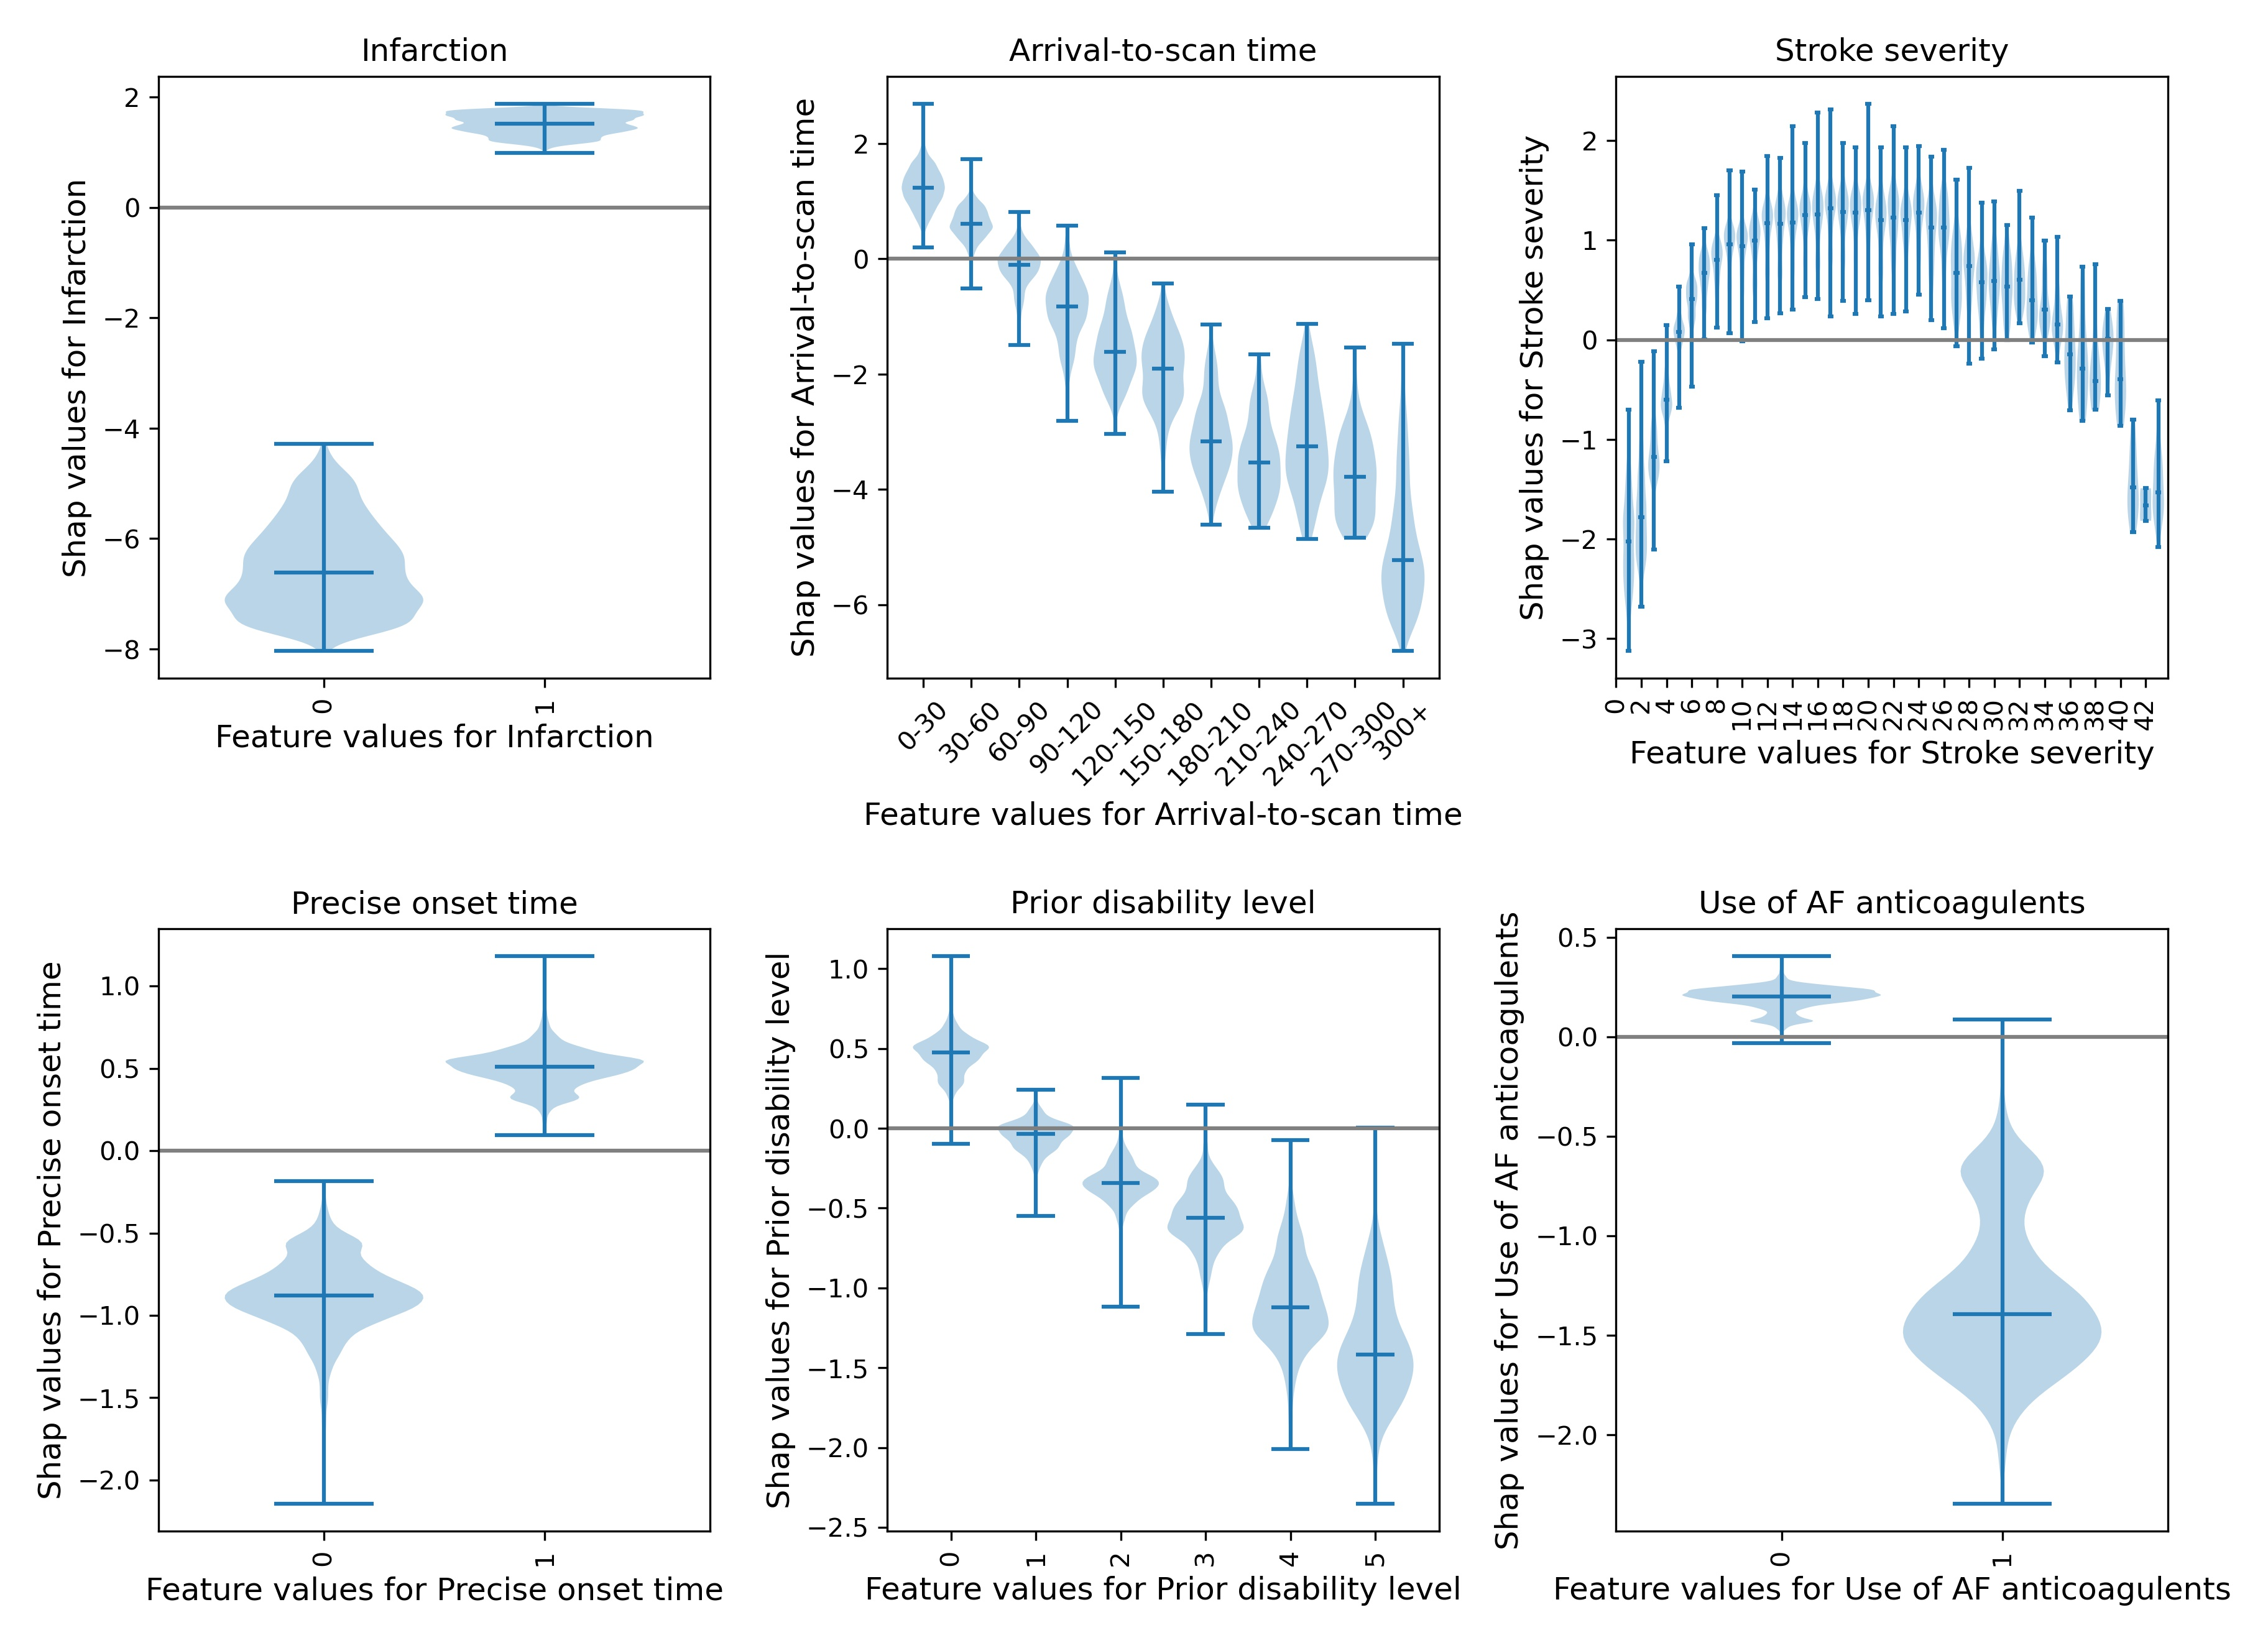
\includegraphics[width=0.78\textwidth]{./images/xgb_thrombolysis_shap_violin.jpg}
\end{center}
\end{frame}

\end{document}

\end{document}



